\documentclass[12pt]{article}

\usepackage{graphicx}
\usepackage{amsmath}
\usepackage{amssymb}
\usepackage{enumerate}
\usepackage{listings}
\usepackage{xcolor}
\usepackage{verbatim}
%%%%%%%%%%%%%%%%%%%%%%%%%%%%%%
\oddsidemargin  0.0in
\evensidemargin 0.0in
\textwidth      6.5in
\headheight     0.0in
\topmargin      0.0in
\textheight     9.0in
\setlength{\parskip}{.7em}
\setlength{\parindent}{0pt}
%%%%%%%%%%%%%%%%%%%%%%%%%%%%%%
\begin{document}
	\title{Quantum Computing: A Guide in English}     
	\author{Struan McDonough}
	\date{\today}
	\maketitle
	
\section{An introduction}

\subsection{Why does this guide exist}

I wrote this guide because while studying Quantum Computing, I found that the notes available to students are inaccessible and rely heavily upon a knowledge of Physics. This document aims to explain the Physics which grounds the course and attempts to make this area of study accessible to Computer Scientists.

\subsection{Transition Systems}

\subsubsection{Definitions}

A transition system can be used to describe an observable system. It's a mathematical way of describing the different states something can take, and how those states can be connected with actions. An action simply takes something, and changes it state from a state $s_1$, to a state $s_2$.

\begin{itemize}
\item A \textbf{state space} is a set $S$ of states the observed system can take.
\item An \textbf{initial state} is a fixed element $s_1 \in S$.
\item A \textbf{current state} is a variable element $s \in S$.
\item A \textbf{action} belongs to a set of possible actions $Act$.
\item A \textbf{transition} is a triple $(s, act, s')$ where $act$ is an action which takes $s$ to the state of $s'$.
\item A \textbf{transition system} $S$ on $(S, Act)$ is a set of transitions built using a state space and a set of Actions $Act$.
\end{itemize}

Usually in Quantum Computing, we assume that there is only ever one action between any two states. Hence we can write a transition as $(s, s')$ as opposed to $(s, act, s')$.

\subsubsection{Example}

If we consider a 32 bit register, we can deconstruct this scenario in terms of a transition system.

\begin{itemize}
	\item The state space is the set of values which can be held in the register
	\item The initial state of a register is what it looks like when it is turned on. In most cases, this is every value in the register taking the value of 0.
	\item The current state is the value held in the register at any given time.
	\item The actions are the set of all machine instructions which can be performed on the register.
	\item The transitions are the set of all possible computation steps (from one state to another using a given instruction).
\end{itemize}

\subsubsection{Deterministic vs Non-Deterministic Behaviour}

We say that an action is \textbf{deterministic} if when repeated, it yields the same result. For example, 1 + 1 always equals 2.

We say that an action is \textbf{non-deterministic} if when repeated, it yields a different result. A fair coin toss is non-deterministic.

\subsubsection{Different Types of Transition Systems}

We can have both \textbf{deterministic transition systems} and \textbf{non-deterministic transition systems}. This is where all of the actions are deterministic or non-deterministic respectively.

A \textbf{Stochastic Transition System} is one in which every transition $(s, s')$ has an associated probability $p(s, s')$. The sum of all transition probabilities leaving a state must equal 1. 

A \textbf{Quantum Transition System} is one in which every transition $(s, s')$ has an associated probability amplitude $\psi(s, s')$.

A \textbf{Probability Amplitude} is a different measurement used to label transitions. These can be turned into probabilities by taking the modulus, and then squaring it. 

\begin{center}
	$\lvert (\psi(s, s')) \rvert^2 = p(s, s')$. 
\end{center}

The probabilities these generate must also equal 1.

\begin{center}
	$\sum_{s'} \lvert \psi(s,s') \rvert^2 = 1$
\end{center}

\subsection{Probability Amplitudes}

In Quantum Systems, we must use Probability Amplitudes to describe changes in a meaningful way. Particles have two main properties which are of interest to us, the information of position and momentum, and the information about the spin of the particle. The position and momentum can change in a continuous way, but the spin of a particle can only take distinct, discrete values. The Mathematics of a Quantum System cannot be expressed using probabilities alone, due to some quite advanced Physics involving Wave Functions and so forth. Normal probabilities can't handle quantum transitions in a meaningful way.

\subsubsection{Sequential Composition}

\begin{center}
	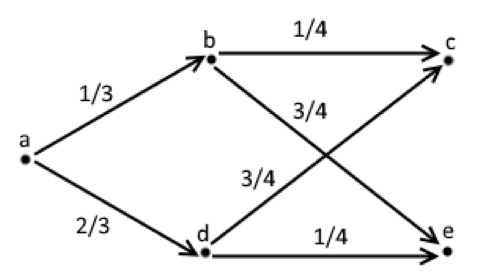
\includegraphics[width=200px]{Fig1}
\end{center}

If we have states $a, b, c$, then to find the probability of going from a to c through b $p(a, b, c)$, we have to compose them. This works by finding all the intermediate steps. $p(a, b) \times p(b, c) = p(a, b, c)$. In the example above, $p(a, b, c) = 1/12$

The same works for probability amplitudes. $\psi(a, b, c) = \psi(a, b) \times \psi(b, c)$.

\subsubsection{Composition of Different Sequences}

This is when we want to get from one state to another, but can use multiple sequences. 

$p(a, b, c) = p(a, b) \times p(b, c)$

$p(a, d, c) = p(a, d) \times p(d, c)$

$p(a, c) = p(a, b, c) + p(a, d, c) = (p(a, b) \times p(b, c)) + (p(a, d) \times p(d, c))$

Stochastic and Quantum Transition systems work in exactly the same way during composition of sequences.

However, when converting the Quantum System back into a Transition System, some odd things can happen!

$p_Q(a, c) = (p_Q(a, b) \times p_Q(b, c)) + (p_Q(a, d) \times p_Q(d, c))$

However, $p_Q(a, b) = |\psi(a, b)|^2$. (By the way, I'm going to stop writing the $\times$ explicitly...)

$p_Q(a,c) = \lvert \psi(a,b)\psi(b,c) + \psi(a,d)\psi(d, c) \rvert^2$

$p_Q(a,c) = \lvert \psi(a,b)\psi(b,c) \rvert^2 + \lvert \psi(a,d)\psi(d,c) \rvert^2 + \psi(a,b)\psi(b,c)\psi^*(a,d)\psi^*(d,c) + \psi^*(a,b)\psi^*(b,c)\psi(a,d)\psi(d,c)$

Now the above looks quite scary, but it's the simple $(ab + cd)^2$ expansion. Also, $\psi*(a,b)$ is the complex conjugate of $\psi(a,b)$.

\section{Linear Algebra}

\subsection{Dirac Notation}

Dirac Notation (Aka Bra-ket) notation is used for describing quantum states. $\lvert x \rangle$ is called a bra, and $\langle y \rvert$ is called a ket. Hence $\langle x \vert y \rangle$ is a bra-ket.

A bra $\langle x \rvert$ denotes a row vector $\begin{bmatrix}x_1 & ... & x_n\end{bmatrix}$.

A ket $\lvert y \rangle$ denotes a column vector $\begin{bmatrix}y_1\\...\\y_n\end{bmatrix}$. 

To save space in documents, we sometimes write a column vector as $\begin{bmatrix}x_1 & ... & x_n\end{bmatrix}^T$, where T stands for transpose. Just imagine rotating it clockwise by 90 degrees.

\subsubsection{Vector multiplication}

There's two main types of vector multiplication: inner product and outer product. 

The inner product is when you multiply a \textbf{bra} by a \textbf{ket} $\langle x \lvert y \rangle$. This returns a scalar (a number), and is calculated by multiplying together each pair of entries at each index, then add up the result.

$ \langle x \lvert y \rangle = \begin{bmatrix}x_1 & ... & x_n\end{bmatrix} \times \begin{bmatrix}y_1\\...\\y_n\end{bmatrix} = x_1y_1 + x_2y_2 + ... + x_ny_n$

The outer product is when you multiply a \textbf{ket} by a \textbf{bra} $\lvert x \rangle \langle y \rvert$. This returns a matrix, and is defined as follows:

$\lvert x \rangle \langle y \rvert = \begin{bmatrix}x_1\\...\\x_n\end{bmatrix} \times \begin{bmatrix}y_1 & ... & y_n\end{bmatrix} = \begin{bmatrix} x_1y_1 & ... & x_1y_n \\ ... & & ... \\ x_ny_1 & ... & x_ny_n\end{bmatrix}$

\subsection{Complex Inner Product Space}

This is a type of set (H) which is defined by the following properties:

\begin{itemize}
	\item Any two vectors in the set are \textbf{commutative under addition}: \\$\lvert x \rangle, \lvert y \rangle \in H \implies \lvert x \rangle + \lvert y \rangle = \lvert x + y \rangle = \lvert y \rangle + \lvert x \rangle \in H$.
	\item Any three vectors in the set are \textbf{associative under addition}: \\$\lvert x \rangle, \lvert y \rangle, \lvert z \rangle \in H \implies (\lvert x \rangle + \lvert y \rangle) + \lvert z \rangle = \lvert x \rangle (\lvert y \rangle + \lvert z \rangle)$
	\item The set \textbf{contains a zero element}, which does nothing when applied to a vector:\\$\underline{0} \in H$ and $\underline{0} + \lvert x \rangle = \lvert x \rangle \in H$
\end{itemize}

\end{document}
